\documentclass{article}
\usepackage[utf8]{inputenc}

% Page setup
\usepackage[a4paper,landscape,margin=2cm]{geometry}
\usepackage{amsmath}

% Typography
\usepackage[scaled]{helvet}
\let\familydefault\sfdefault

\usepackage[usenames,svgnames]{xcolor}
\usepackage{tikz,pgfplots}
\usetikzlibrary{positioning,arrows,intersections}

\definecolor{colortext}     {RGB}{29 ,29 ,27 }

\begin{document}
\pagestyle{empty}
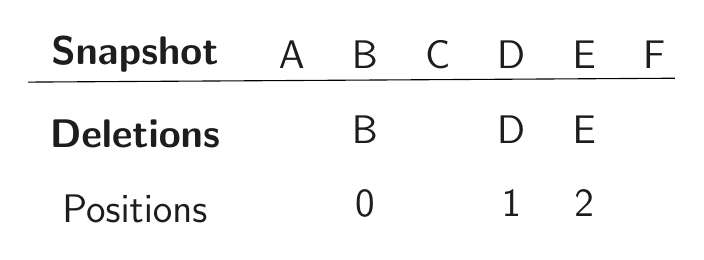
\begin{tikzpicture}[
    node distance = 1em, auto,
    font={\Large\itshape},
    txt/.style={text=colortext,font={\Large},align=center},
    txtbf/.style={txt,font={\Large\bfseries},text width=7em},
]

    \node[txtbf]                   (snapshot) {Snapshot};
    \node[txt,right=of snapshot]   (sa)       {A};
    \node[txt,right=of sa      ]   (sb)       {B};
    \node[txt,right=of sb      ]   (sc)       {C};
    \node[txt,right=of sc      ]   (sd)       {D};
    \node[txt,right=of sd      ]   (se)       {E};
    \node[txt,right=of se      ]   (sf)       {F};
    
    \draw (snapshot.south west) -- (sf.south east);
    
    \node[txtbf,below=of snapshot] (del)      {Deletions};
    \node[txt,below=of sb      ]   (db)       {B};
    \node[txt,below=of sd      ]   (dd)       {D};
    \node[txt,below=of se      ]   (de)       {E};
    
    \node[txt,below=of del]        (del)      {Positions};
    \node[txt,below=of db      ]   (dbp)      {0};
    \node[txt,below=of dd      ]   (ddp)      {1};
    \node[txt,below=of de      ]   (dep)      {2};

\end{tikzpicture}
\end{document}
